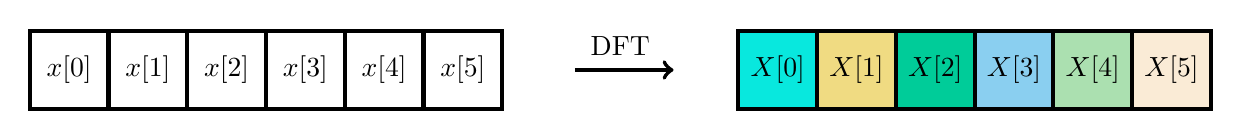
\begin{tikzpicture}
\definecolor{brightturquoise}{rgb}{0.03, 0.91, 0.87}
\definecolor{buff}{rgb}{0.94, 0.86, 0.51}
\definecolor{caribbeangreen}{rgb}{0.0, 0.8, 0.6}
\definecolor{celadon}{rgb}{0.67, 0.88, 0.69}
\definecolor{darktangerine}{rgb}{1.0, 0.66, 0.07}
\definecolor{darkviolet}{rgb}{0.58, 0.0, 0.83}
\definecolor{deepskyblue}{rgb}{0.0, 0.75, 1.0}
\definecolor{amber(sae/ece)}{rgb}{1.0, 0.49, 0.0}
\definecolor{antiquewhite}{rgb}{0.98, 0.92, 0.84}
\definecolor{applegreen}{rgb}{0.55, 0.71, 0.0}
\definecolor{babyblue}{rgb}{0.54, 0.81, 0.94}



% 6-point time domain signal
\draw[thick,line  width =1.5pt]  (1,3) rectangle (2,2);
\draw[thick,line  width =1.5pt]  (2,3) rectangle (3,2);
\draw[thick,line  width =1.5pt]  (3,3) rectangle (4,2);
\draw[thick,line  width =1.5pt]  (4,3) rectangle (5,2);
\draw[thick,line  width =1.5pt]  (5,3) rectangle (6,2);
\draw[thick,line  width =1.5pt]  (6,3) rectangle (7,2);
\node at (1.5,2.5) {$x[0]$};
\node at (2.5,2.5) {$x[1]$};
\node at (3.5,2.5) {$x[2]$};
\node at (4.5,2.5) {$x[3]$};
\node at (5.5,2.5) {$x[4]$};
\node at (6.5,2.5) {$x[5]$};

% DFT arrow
\node (v1) at (7.8,2.5) {};
\node (v2) at (9.3,2.5) {};
\draw[thick, ->,line  width =1.5pt]  (v1) edge (v2);
\node at (8.5,2.8) {DFT};

% 6-point frequency signal
\draw[thick,fill=brightturquoise,line  width =1.5pt]  (10,3) rectangle (11,2);
\draw[thick,fill=buff,line  width =1.5pt]  (11,3) rectangle (12,2);
\draw[thick,fill=caribbeangreen,line  width =1.5pt]  (12,3) rectangle (13,2);
\draw[thick,fill=babyblue,line  width =1.5pt]  (13,3) rectangle (14,2);
\draw[thick,fill=celadon,line  width =1.5pt]  (14,3) rectangle (15,2);
\draw[thick,fill=antiquewhite,line  width =1.5pt]  (15,3) rectangle (16,2);
\node at (10.5,2.5) {$X[0]$};
\node at (11.5,2.5) {$X[1]$};
\node at (12.5,2.5) {$X[2]$};
\node at (13.5,2.5) {$X[3]$};
\node at (14.5,2.5) {$X[4]$};
\node at (15.5,2.5) {$X[5]$};
\end{tikzpicture}